\documentclass{zjureport}
% =============================================
% Part 1 Edit the info
% =============================================

\newcommand{\coursenum}{0205740001}
\newcommand{\coursename}{金融统计软件应用(英文版)}
\newcommand{\lecturer}{黄嘉平}
\newcommand{\grade}{1}
\newcommand{\studentnum}{2017022002}
\newcommand{\yourname}{陈明}
\newcommand{\major}{17级金融学}
\newcommand{\firstyear}{一八}
\newcommand{\secondyear}{一九}
\newcommand{\term}{二}
\newcommand{\titleofpaper}{R Final Report}
\usepackage{multicol}
\usepackage{graphicx}
\usepackage{graphics}
\usepackage{amssymb}  
\usepackage{amsmath}
\usepackage{float}
\usepackage{bm}  
\usepackage{booktabs}
\usepackage{float}
\usepackage{subfigure}

% =============================================
% Part 1 Main document
% =============================================
\begin{document}
\begin{center}
	\Huge{深圳大学考试答题纸}\\
	\large(以论文、报告等形式考核专用)\\
	\large 二O \underline\firstyear ~二O \underline\secondyear 学年度第 \underline\term  学期
\end{center}

\thispagestyle{empty}%如果注释掉,上面会出现姓名学号等

\begin{table}[!htbp]
  \centering
  \begin{tabular*}{\linewidth}{llllllll}
    课程编号: & \underline\coursenum   & 课程名称: & \underline\coursename   & 主讲教师: &  \underline\lecturer &
    评分: & \_\_ \\  学号:&\underline\studentnum  & 姓名:& \underline\yourname & 专业年级: & \underline\major
  \end{tabular*}
\end{table}

\begin{table}[h] 
	\centering  
			\begin{tabular}{|c c c c c c c c c c c c c c c c c c c c c c c c c c c c c c c c c c c|}   % c 表示表格中的文字居中
			\hline
				\large 教师评语: & & & & &  & & & & &  & & & & &  & & & & & & &  & & & & & & & &  & & &  &\\
				 & & & & &  & & & & &  & & & & &  & & & & & & &  & & & & & & & &  & & &  &\\
				 & & & & &  & & & & &  & & & & &  & & & & & & &  & & & & & & & &  & & &  &\\
				 & & & & & & & & & &  & & & & &  & & & & & & &  & & & & & & & &  & & &  &\\
			\hline
			\end{tabular}
\end{table}

\large 题目:\underline\titleofpaper

% =============================================
% Part 2 Main document
% =============================================
\tableofcontents
\newpage
\section{Part 1}
\subsection{Report descriptive statistics of the data set obtained in (a).}
The report on descriptive statistics is shown in table \ref{tab1} and table \ref{tab2}.
\begin{table}[htbp]
	\centering
	\caption{Descriptive Statistics 1}
	\begin{tabular}{lrrrrr}
		\toprule[1.5pt]
		& \multicolumn{1}{l}{Wr.Hnd} & \multicolumn{1}{l}{NW.Hnd} & \multicolumn{1}{l}{Pulse} & \multicolumn{1}{l}{Height} & \multicolumn{1}{l}{Age} \\
		\toprule[1.5pt]
		Min.  & 13.00 & 12.50 & 35.00 & 152.00 & 16.92 \\
		1st Qu. & 17.50 & 17.50 & 66.75 & 165.00 & 17.67 \\
		Median & 18.50 & 18.50 & 72.00 & 170.60 & 18.58 \\
		Mean  & 18.80 & 18.73 & 74.02 & 172.50 & 20.43 \\
		3rd Qu. & 20.00 & 20.00 & 80.00 & 180.00 & 20.17 \\
		Max.  & 23.20 & 23.50 & 104.00 & 200.00 & 70.42 \\
		\toprule[1.5pt]
	\end{tabular}%
	\label{tab1}%
\end{table}%

\begin{table}[htbp]
	\centering
	\caption{Descriptive Statistics 2}
	\begin{tabular}{rrrrrlr}
		\toprule[1.5pt]
		\multicolumn{1}{l}{Sex} & \multicolumn{1}{l}{W.Hnd} & \multicolumn{1}{l}{Fold} & \multicolumn{1}{l}{Clap} & \multicolumn{1}{l}{Exer} & Smoke & \multicolumn{1}{l}{M.I} \\
		\toprule[1.5pt]
		\multicolumn{1}{l}{Female:84} & \multicolumn{1}{l}{Left:12} & \multicolumn{1}{l}{L on R :72} & \multicolumn{1}{l}{Left: 28} & \multicolumn{1}{l}{Freq:85} & Heavy:  7 & \multicolumn{1}{l}{Imperial: 58} \\
		\multicolumn{1}{l}{Male:84} & \multicolumn{1}{l}{Right:156} & \multicolumn{1}{l}{Neither: 8} & \multicolumn{1}{l}{Neither: 33} & \multicolumn{1}{l}{None:14} & Never:134 & \multicolumn{1}{l}{Metric  :110} \\
		&       & \multicolumn{1}{l}{R on L :88} & \multicolumn{1}{l}{Right  :107} & \multicolumn{1}{l}{Some:69} & Occas: 13 &  \\
		&       &       &       &       & Regul: 14 &  \\
		\toprule[1.5pt]
	\end{tabular}%
	\label{tab2}%
\end{table}%


\subsection{Use boxplot to show the distributions of the height of male and female students.}
The distributions of the height of male and female students are illustrated in figure \ref{distribution1}. 

\begin{figure}[!ht]
	\centering
	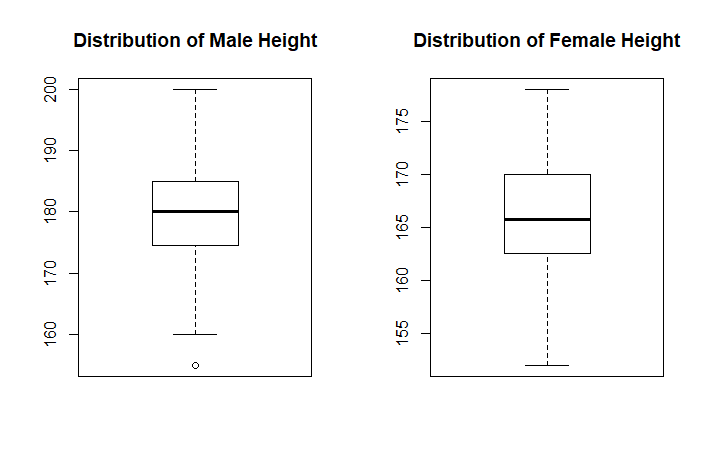
\includegraphics[width=0.8\textwidth]{Rplot.png}
	\caption{Distribution of Heights}
	\label{distribution1}
\end{figure}

\subsection{Which numerical variables might have an influence on the student's pulse?}
\begin{table}[htbp]
  \centering
  \caption{Correlations and P-Values }
      \begin{tabular}{lrr}
                \toprule[1.5pt]
          & \multicolumn{1}{l}{cor(y,x)} & \multicolumn{1}{l}{P-value} \\
          \toprule[1.5pt]
    Pulse and Age & -0.288 & 0.1144 \\
    Pulse and Height & -0.08326 & 0.283 \\
    Pulse and Wr.Hnd & -0.01382 & 0.859 \\
    Pulse and Sex & 0.064165 & 0.409 \\
    Pulse and Sex & -0.04239 & 0.585 \\
    Pulse and Fold & -0.13951 & 0.071 \\
    Pulse and Exer & -0.05905 & 0.447 \\
    Pulse and Clap & 0.198341 & 0.01 \\
    Pulse and W.Hnd & 0.05421 & 0.485 \\
              \toprule[1.5pt]
        \end{tabular}%
  \label{cor}%
\end{table}%
To indentify variables that have influence on students' pulse, we can first calculate the correlations between Pulse and independent variable, and then conduct correlation test to make sure both variables are significantly correlated. Table \ref{cor} shows only ''Clap'' is significantly corelated with ''Pulse'' with a correlation of .198341. Hence we can conclude that ''Clap'' might be the factor that significantly influences pulse.

\subsection{Is the probability of a student clapping his/her left hand on top less than 0.2?}
To make sure whether the probability of a student clapping hand on top less than 0.2, we can use prop.test funtion to conduct proportion test. The null hypothesis is that “The probability of a student clapping his/her left hand on top greater than or equal to 0.2”, and the alternative hypothesis is that “probability of a student clapping his/her left hand on top less than 0.2”. The p-value is 0.1626 in this case, which suggests that we cannot reject the null hypothesis at .1 level of significance. Therefore we can infer that the probability of a student clapping his/her left hand on top is equal to or greater than 0.2.
\subsection{Is the span of the writing hand in general larger than the span of the non-writing hand?}
To make sure whether the span of the writing hand in general larger than the span of the non-writing hand, we can make a hypothesis test. The null hypothesis is ‘the span of the writing hand is in general smaller than or equal to the span of the non-writing hand’, and the alternative hypothesis is ‘the span of the writing hand is in general larger to the span of the non-writing hand’. With a p-value of 0.3696, the hypothesis test result suggests that we cannot reject the null hypothesis. Therefore the the span of the writing hand is in general equal to or smaller than the span of the non-writing hand.

\section{Part 2}
\subsection{According to CLT, what is the approximated distribution of the sample means?}
According to CLT, the means of the sample tends towards a normal distribution. The approximated distribution of the sample means is normal distribution.


\subsection{Draw the density plots of the sample means and its approximated distribution on one graph}
The density plots are demonstrated in figure \ref{density plots}.
\begin{figure}[!ht]
	\centering
	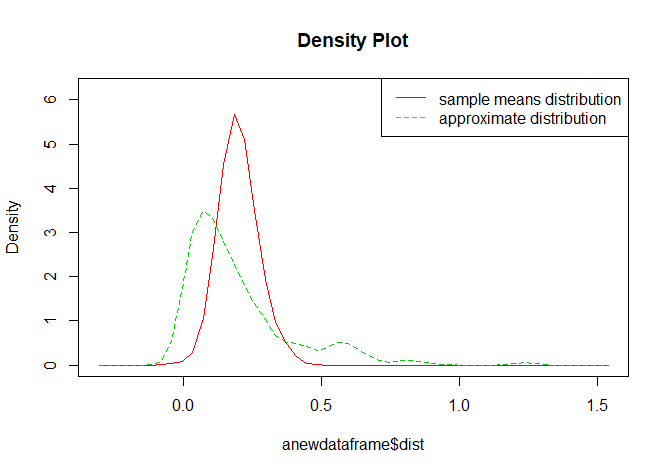
\includegraphics[width=0.8\textwidth]{Rplot01.png}
	\caption{Density Plot}
	\label{density plots}
\end{figure}


\subsection{Show the qq plot of the distribution of the sample means}
	The QQ plot of the distribution of the sample means is demonstrated in figure \ref{QQ plot}.
\begin{figure}[!ht]
	\centering
	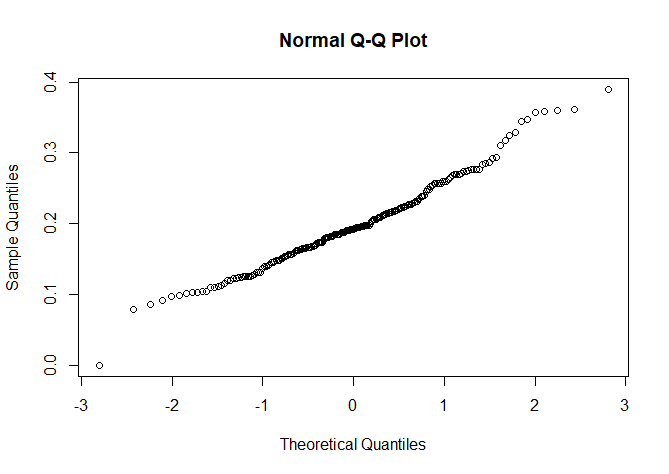
\includegraphics[width=0.8\textwidth]{Rplot02.png}
	\caption{QQ Plot}
	\label{QQ plot}
\end{figure}

\subsection{What conclusion can you draw from this simulation?}
From the density plot, we can know that the sample means distribution tends towards normal distribution as the sample means number gets greater. From QQ plot, we can also observe that the points fall on the straight 45-degree line, which suggests that the residual values are normally distributed with a mean of 0. Hence the sample means are normally distributed.

\section{Part 3}
\subsection{Draw 5000 random samples of X}
The random samples generated are omitted here.

\subsection{Given $\alpha$ = 0.05, find the VaR of the samples obtained in 3.1}
Since VaR denotes the critical value L such that $P(X>L)=\alpha P(X>L)=\alpha$ ,to find the VaR of the samples, we first need to sort the array of the change of the stock price ascendingly. Then we can use quantile function to find out the change value situated at given $\alpha$. The VaR is -2.188176. (Note that as the values of samples vary each time we rerun the code, the VaR is unlikely to remain the current value)

\subsection{Find the CVaR of the samples obtained in 3.1}
CVaR is the average loss over a specified time period of unlikely scenarios beyond the confidence level. By calculating the arithmetic mean of rate of return under the critical value L, we can find the CVAR is -3.034234. (Note that as the values of samples vary each time we rerun the code, the CVaR is unlikely to remain the current value)



\section{Part 4}
\subsection{Report on  data exploration}
We can use Distribution, pie charts, and boxplots, etc to explore on the data.

\begin{figure}[!ht]
	\centering
	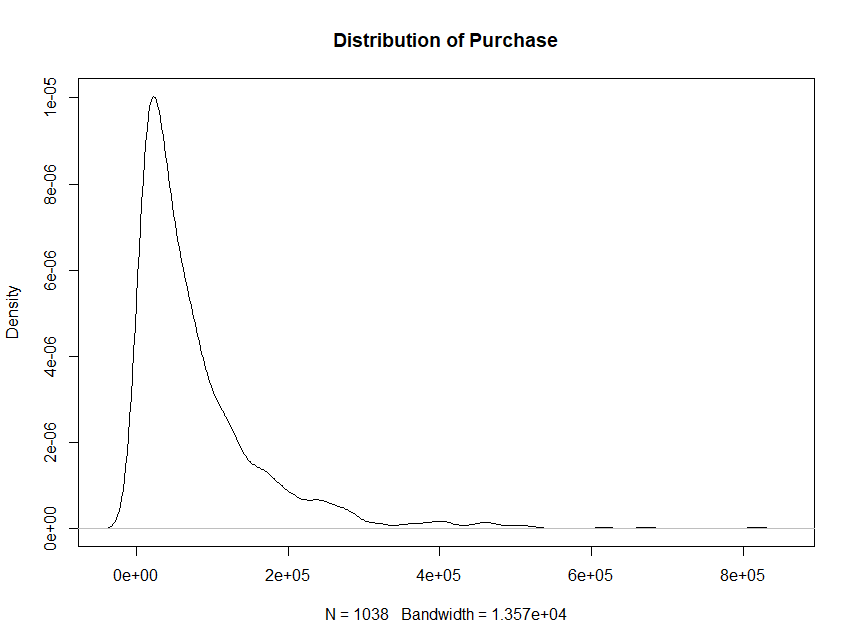
\includegraphics[width=.8\textwidth,height=.5\textwidth]{Rplot11.png}
	\caption{Distribution of Purchases Amount}
\end{figure}

\begin{figure}[H]
	\centering
	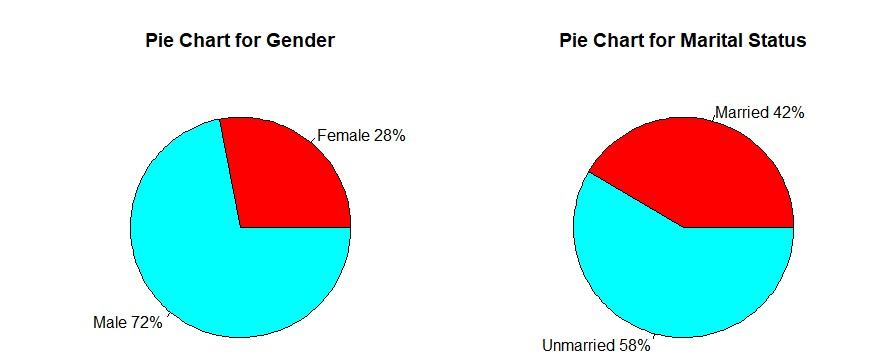
\includegraphics[width=1\textwidth]{Rplot04.jpg}

	\centering
	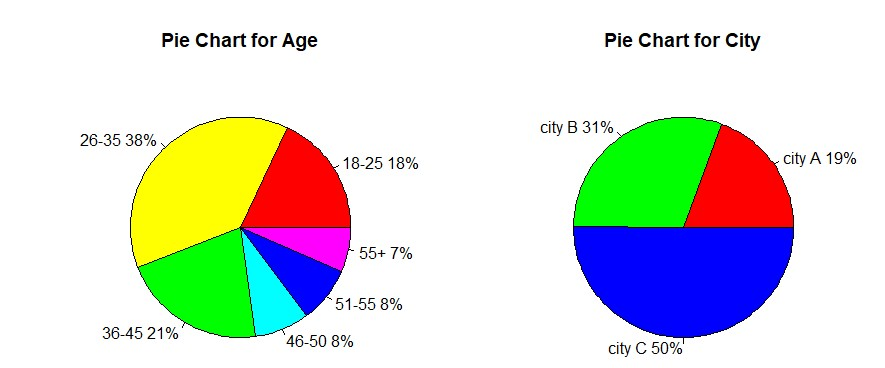
\includegraphics[width=1\textwidth]{Rplot05.jpg}

	\centering
	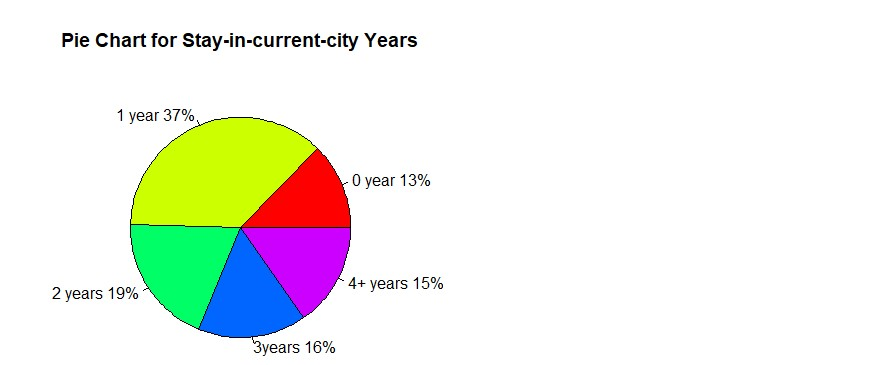
\includegraphics[width=1\textwidth]{Rplot06.jpg}
	\caption{Pie Charts For Other Variables Distributions}
\end{figure}

\begin{figure}[H]
	\centering
	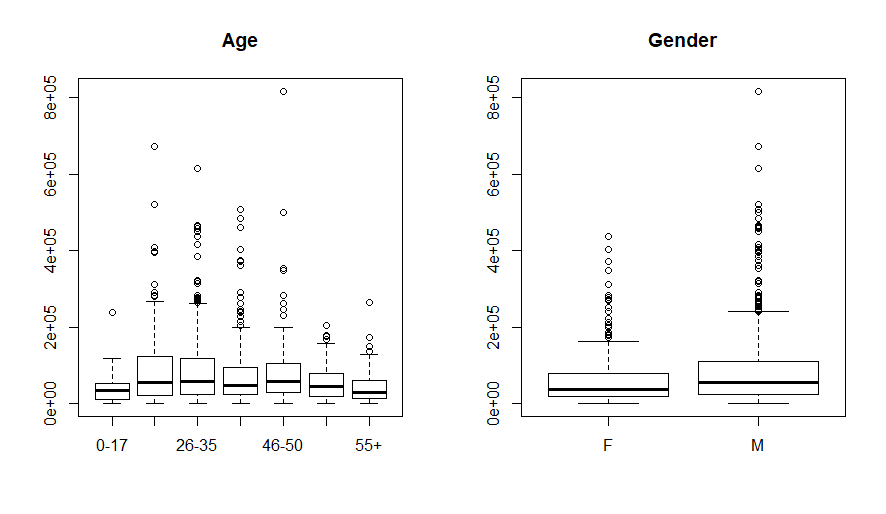
\includegraphics[width=1\textwidth,height=.45\linewidth]{Rplot07.png}

	\centering
	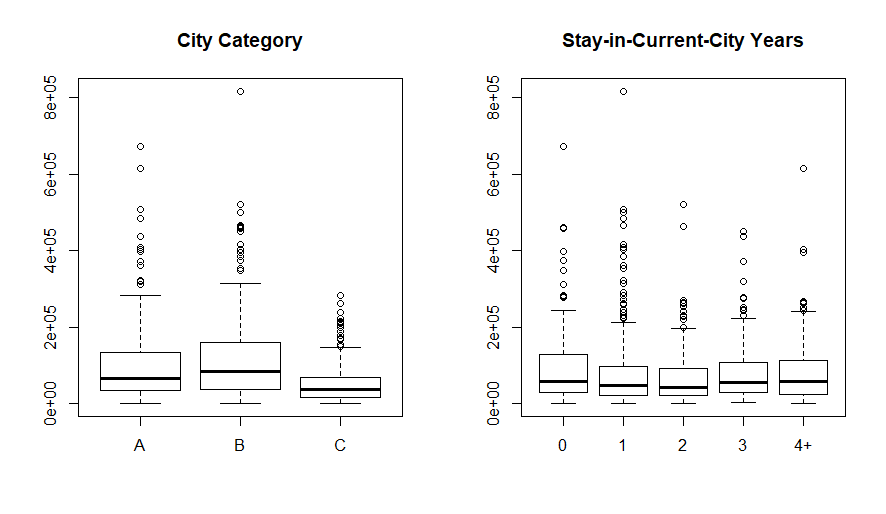
\includegraphics[width=1\textwidth,height=.45\linewidth]{Rplot08.png}

	\centering
	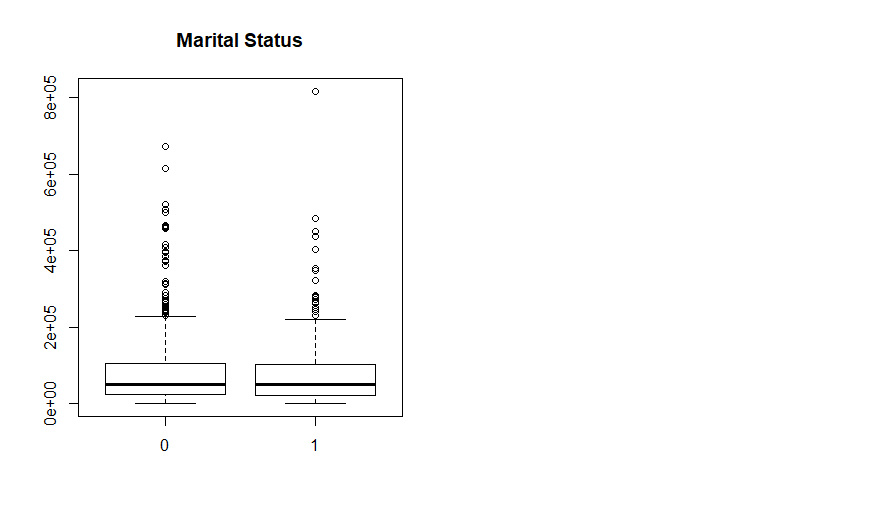
\includegraphics[width=1\textwidth,height=.45\linewidth]{Rplot09.png}
	\caption{Box Plots For Other Variables Distributions}
\end{figure}

\begin{table}[htbp]
	\centering
	\caption{Correlation Coefficients by Kendall Method}
	\begin{tabular}{ccccc}
			\toprule[1.5pt]
		cor(y,x0) & cor(y,x1) & cor(y,x2) & cor(y,x3) & cor(y,x4) \\
		\toprule[1.5pt]
		0.0287828 & -0.2512844 & -0.10772 & 0.011602 & -0.01244 \\
		\toprule[1.5pt]
	\end{tabular}%
	\label{tab:addlabel}%
\end{table}%



\subsection{Report on modeling (baseline model and alternatives)}
We can take the independent varibles with the greatest correlation coefficient as the baseline model. Therefore, we begin constructing the regression model with 'city catergory' as the only independet variable. By adding independent values step by step in order of their correlation coefficients values. By adding independent variables step by step, we find that 'marital status' is not significantly related to purchases amount.  In addition, we can also evaluate the model with ''StepAIC'' function. The result complies with the fitted model, lending supports for the validity of the fitted model. Hence we construct the fitted model with the remaining independent variables. The equation of the fitted model is:
\begin{equation}
	y = 83820 - 55169x_{1} + 25064x_{2} + 37766x_{3} - 20332x_{4} - 27843x_{5} 
\end{equation} 
in which $x_{i}$ are dummy varibles of certain factors. 
\subsection{Report on results and interpretation of the fitted model}
Results of the fitted model have been demonstrated in table \ref{fitted model} and subsection 4.2.  From table \ref{fitted model}, we find that Purchases Amount is significantly related to 'City Category', 'Age', 'Gender', and 'Stay-in-current-city Years'. From the results we can conclude that the following factors significantly affect purchase amount: whether the customer live in city C, whether the customer is male, whether the customer is aged between 46 and 50, whether the customer stays in current city for 1 or 2 years. The fitted model implies that, when the aforementioned conditions are met, the customer is more likely to spend more on purchasing.

\begin{table}[htbp]
	\centering
	\caption{P-values and Coefficients of The Fitted Regression Model}
    \begin{tabular}{lrrr}
    	\toprule[1.5pt]
	& \multicolumn{1}{l}{$Pr(>|t|)$} &       & \multicolumn{1}{l}{Coefficients} \\
	\hline
	(Intercept) & 8.35E-08 & \multicolumn{1}{l}{***} & 83820 \\
	newdata\$City\_CategoryB & 0.2375 &       & 8792 \\
	newdata\$City\_CategoryC & 6.07E-15 & \multicolumn{1}{l}{***} & -55169 \\
	newdata\$GenderM & 1.35E-05 & \multicolumn{1}{l}{***} & 25064 \\
	newdata\$Age18-25 & 0.0887 & \multicolumn{1}{l}{.} & 24030 \\
	newdata\$Age26-35 & 0.0654 & \multicolumn{1}{l}{.} & 24692 \\
	newdata\$Age36-45 & 0.1004 & \multicolumn{1}{l}{.} & 22770 \\
	newdata\$Age46-50 & 0.0161 & \multicolumn{1}{l}{*} & 37766 \\
	newdata\$Age51-55 & 0.8677 &       & 2593 \\
	newdata\$Age55+ & 0.8107 &       & 3890 \\
	newdata\$Stay\_In\_Current\_City\_Years1 & 0.0154 & \multicolumn{1}{l}{*} & -20332 \\
	newdata\$Stay\_In\_Current\_City\_Years2 & 0.0028 & \multicolumn{1}{l}{**} & -27843 \\
	newdata\$Stay\_In\_Current\_City\_Years3 & 0.0728 & \multicolumn{1}{l}{.} & -17374 \\
	newdata\$Stay\_In\_Current\_City\_Years4+ & 0.114 &       & -15446 \\
	\toprule[1.5pt]
\end{tabular}%
	\label{fitted model}%
\end{table}
	
\subsection{Report on model assumptions}
In Q-Q graph, points basically cluster around the line, which proves that the assumption of Normality is satisfied; there is no reason to assume any of the independents are correlated. Therefore, the assumption of Independence is satisfied; from graph one, we can observe that residuals have no systematic relationship between residuals and the predicted values. In the Residuals vs. Fitted graph, you see clear evidence of a straight relationship, and hence the model well captures systematic variance in the data, thereby proves that the assumption of Linearity is satisfied; the Scale-Location graph shows that the points form a random band around the horizontal line. Hence the assumption of Homoscedasticity is satisfied. 
\begin{figure}[H]
	\centering
	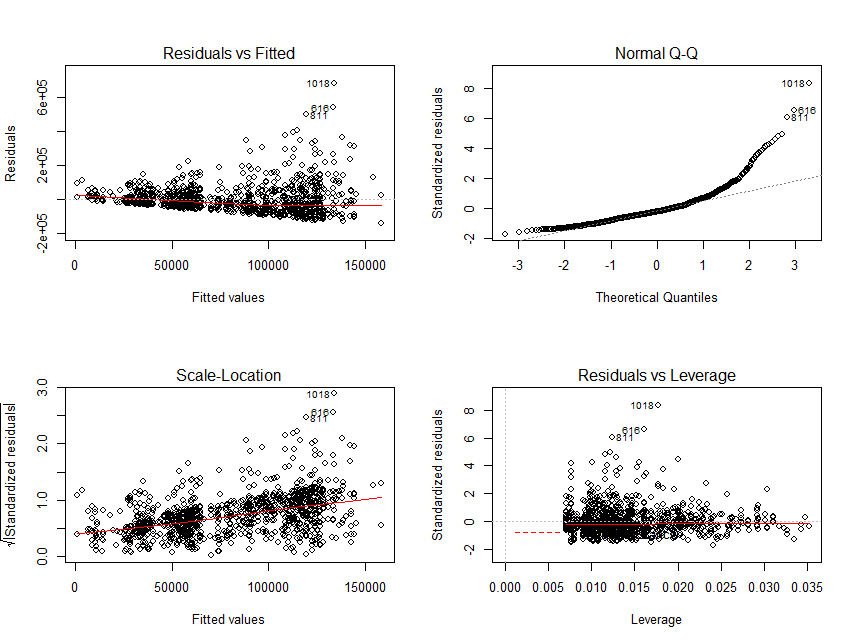
\includegraphics[width=1\textwidth]{Rplot10.png}
	\caption{Diagnostic plots}
\end{figure}


\end{document}
